% see A1.4
\chapter{Planen}
Die Zeitplanung wird in der Abbildung \ref{fig:timeplan} oberhalb gezeigt. Die restlichen Aspekte der Planung sind in diesem Kapitel dokumentiert.

\section{Anwendungsfälle}

\section{Datenmodell}
\begin{figure}[H]
  \begin{center}
    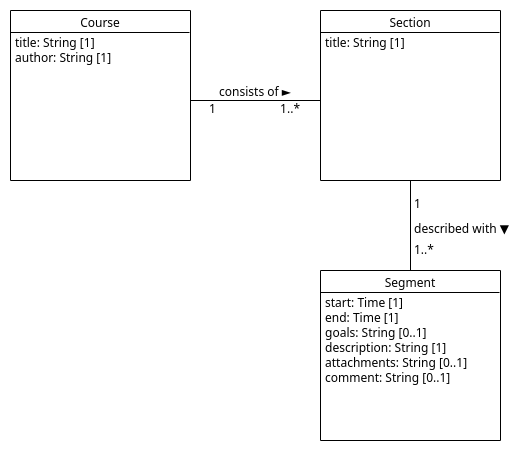
\includegraphics[width=0.8\textwidth]{../res/datamodel.png}
  \end{center}
  \caption[\enquote{Datenmodell} visualisiert mit Umlet]{Datenmodell}
  \label{fig:datamodel}
\end{figure}

\section{Testkonzept}
Das Testkonzept beschreibt, wie und mit welchen Werkzeugen das Resultat auf seine Richtigkeit kontrolliert wird.

\subsection{Testmethoden}

\subsection{Testmittel}